\chapter{Deep Learning for Stock Market Prediction: Forecasting and Decision-Making using GRU, CNN, and LSTM Network}

\textbf{Abstract: }
The stock market is a volatile and complex system where predicting price movements accurately and making informed decisions can be extremely difficult. Montalvo et al. (2018) Cnn Prof Cnn This study focuses on making stock prediction tasks using deep learning when using three different designs of deep learning (DL) architectures (Gated Recurrent Unit (GRU), Convolutional Neural Network (CNN) and Long Short-term Memory (LSTM) networks) and historical data. Our proposed methodology consists of a live dynamic backtesting heuristic which pre-processes time-series data with per-ticker scaling, hyperparameter-tuning through Keras Tuner, combined ensemble model fitting, trading signal generation and finally performance evaluation against various metrics like Maximum Drawdown, Sharpe ratio, final balance. This Python implementation of the framework, validated in TradingView's PineScript, outperforms traditional technical indicator strategies akin to the "Total 20 Stock Marker Strategy [First Research Project]" project (Profit: \$38.62 USD) leveraging the Momentum indicator.

The study utilizes a `DataProcessor` class to generate sequences with a tunable lookback period (optimized within 10 to 120 days), build GRU, CNN, and LSTM models through a `ModelFactory`, and architectures tuning is performed with a `HyperparameterTuner`. Prediction are ensembled by a `CombinedModel`, decision making is supported by a `SignalGenerator` and performance analysis is covered by a `PerformanceAnalyzer`. Experimental case studies validate the framework's versatility with the optimal lookback time selected for minimizing the mean square error in the validation data, as well as the predicted prices, signals and portfolio balances. DL performance versus that of technical indicators is then compared, and future research is proposed in hybrid systems like technical indicators augmented with DLlike data. This paper provides a new framework to connect DL forecasting with applications in trading which has been underexplored in the literature, thus, fills in the missing link of real-time adaptablility and risk management. Future developments may use multi-features as input and include short positionnbsp; to make the model more robust.


\section{Introduction}
Trained on data that continues until October 2023, the stock market is an ever-evolving stage that is dynamic in its uncertainty, with investors and traders alike striving to harness the descriptive power of the past in order to predict price movements and guide their decisions. Traditional methods, like technical analysis through the lens of Moving Average Convergence Divergence (MACD) or Relative Strength Index (RSI) indicators, have historically been go-to alternatives for spotting trends and reversals. But, the introduction of deep learning (DL) has changed the game by providing more complex models that can model non-linear relations and capture long-term dependencies in time-series data. In this article, we propose a new framework called "Stock Market Prediction: Forecasting and Decision-Making using GRU, CNN, and LSTM Networks" that is aimed at predicting stock prices and providing trading signals, which we focus on for S\&P500 Corporation (GSPC), a volatile tech giant that is impacted by both GPU innovations and AI advancements.

This thesis was stimulated by the limitations of static technical indicators strategies as seen from the "Total 20 Stock Marker Strategy" project where indicators such as Momentum gave a profit of 38.62 USD but could not adapt to changing market conditions. Deep learning (DL) approaches, such as Gated Recurrent Unit (GRU), Convolutional Neural Network (CNN), and Long Short-Term Memory (LSTM) networks, provide a data-driven alternative by discovering complex patterns from raw price information. Thus, GSPC’s price dynamics characterized by large trending movements and volatility are perfectly aligned with these models, making it a strong candidate for an advanced forecasting method. This project incorporates a back-testing system that is dynamic, preprocessing data, hyperparameter tuning, ensemble training, and performance evaluation so that we can connect between theoretical prediction and real-life trading experiences.

There are also several important challenges to tackle in stock prediction that the proposed framework can address. Firstly, it addresses data non-stationarity through per-ticker scaling with MinMaxScaler, meaning it normalizes the price range on a per stock basis. Secondly, it tunes the lookback period (10 to 120 days) to find the relevant historical context, which is an important hyperparameter in the context of time-series forecasting. Thirdly, it utilizes hyperparameter tuning with Keras Tuner to improve the model performance considering the black box nature of DL. Finally, it fuses predictions from GRU, CNN, and LSTM, to diminish the learning biases of individual architectures, following recent research on ensemble learning-based approaches.

The two-fold objectives of this study are to predict GSPC stock prices with high accuracy, and then translate the predictions into actionable trading decisions. The backtesting element, setup with a \$5,000 balance and \$0.01 transaction cost, simulates the conditions of real world trading, and key statistics such as maximum drawdown and Sharpe ratio give a solid assessment. This builds on my previous technical indicator project comparing DL against best indicators (e.g. Momentum, VWMA) and hybrid approaches. Therefore, with a consistent integration with TradingView’s PineScript for visual validation, the framework becomes practical for trader.

The importance of this thesis is that it adds framework to quantitative finance. This framework is a scalable tool for stock prediction, utilizing GRU efficiency, LSTM memory and CNN pattern recognition. The model fills existing gaps in literature including real-time adaptability, comprehensive risk assessment, and provides a starting point to explore further enhancements, such as multi-feature inputs and short-selling. With the growing complexity of financial markets, driven by algorithms and high-frequency data, such a DL-based approach should prove instrumental. This study not only contributes to the theoretical knowledge of DL in finance, but also provides a useful tool for traders with applications applicable to a wide variety of assets.

\section{Related Works}

Investors can't trust that they can guess when to buy/sell as stock markets have always been and always will be unpredictable. Yet the creation of traditional technical indicators (i.e., Moving Average Convergence Divergence (MACD), Relative Strength Index (RSI)) based on stock unpredictability was also ineffective to suggest predictability; for example, in our "Total 20 Stock Marker Strategy" project, one of the more successful indicators was Momentum which yielded a modest \$38.62 in profit. Yet by employing deep learning (DL) models like GRU, CNN, and Long LSTM, a statistically driven, empirical approach can be created to identify, for example, nonlinear trends, and long-term dependencies that might occur within a finite financial timeseries. Therefore, we completed "Deep Learning for Stock Market Prediction: Forecasting and
Decision-Making using GRU, CNN, and LSTM Network" to develop a custom framework to assess stock behavior with buy/sell recommendations for S\&P500 (GSPC), a technology stock with high volatility dependent on recent advancements in financial AI technology.

Recent research underscores the strengths of GRU, CNN, and LSTM in quantitative finance. GRUs, known for computational efficiency, have shown high accuracy in stock index prediction with reduced training time \cite{gru_stock_efficiency_2023}. LSTMs, adept at capturing long-term dependencies, achieve R² values above 0.94 on datasets like S\&P 500 \cite{lstm_sp500_r2_2022}. CNNs, when combined with LSTM or GRU, excel in extracting local patterns, with models like CNN-BiSLSTM reducing mean square error by 30\% \cite{cnn_bislstm_mse_2024}. Research on Bitcoin \cite{bitcoin_forecasting_2024} and Nifty 50 \cite{nifty50_dl_2025} highlights DL’s forecasting capabilities, while multimodal models integrating sentiment data improve trend prediction \cite{multimodal_sentiment_2023}. Hybrid frameworks, such as FS-CNN-BGRU \cite{fs_cnn_bgru_2023} and CNN-GRU-AM \cite{cnn_gru_am_2024}, further enhance accuracy through feature selection and attention mechanisms, achieving MAPE as low as 1.43\%. Additional studies on IBM \cite{ibm_dl_case_2022} and investment strategies \cite{investment_dl_2023} reinforce DL’s potential in trading applications. However, gaps remain in real-time adaptability, comprehensive risk assessment (e.g., Value at Risk), and practical backtesting for volatile stocks like NVDA.

These gaps are filled in this work as an ensemble of GRU, CNN, and LSTM is built. The `MinMaxScaler` scales ticker-by-ticker to reduce non-stationarity in addition to the assessed lookback windows (10-120 days) and hyperparameters optimized through `KerasTuner` for a more palatable model. Creating an ensemble minimizes the individual biases as it relies on GRU's speed, LSTM's memory of the past, and CNN's ability to extract features. An adaptive backtesting strategy is created which applies a fixed equity of \$5,000 and a \$0.01 transaction fee per trade to force buy and sell transactions to take long/short positions when the index predictions increase/decrease while measuring effectiveness against maximum drawdown, Sharpe ratio, and significance tests post-hoc. The ability to convert time-series results into PineScript on TradingView provides a visual representation of performance over time, creating an aesthetic framework for any trader's platform. Ultimately, predicting GSPC through this framework provides a consistent and fluid approach for such inherently volatile stocks, outperforming any constant based on static Technical Indicators.

There will be more time to influence future efforts more constructively. We will see that overall, adding in volume and sentiment are at many stages, they will provide significant ability to adapt and improve the predictive accuracy of algorithms. A backtest which (i) allows short selling, (ii) includes various asset classes and (iii) uses a more sophisticated risk metric (such as Value at Risk (VaR)) will be more widely applicable and more stable than one that does not. So this is an evolution of deep learning in quantitative finance, their theoretical forecasting and tool making, trading on one side, and a project on the other. We will update the information on DL algorithmic patterns based on the characteristics of the algorithm, as one of the pioneering papers outlining future innovations of DL in algorithmic trading and high-frequency data activation.

\section{Methodology}
As a progressive guide, the methodology of this project will cover the steps followed to build an ensemble of Deep learning (DL) model and use the target sequence to predict S\&P500 (GSPC) stock prices and generate actionable trading signals. In this section, the data collection, preprocessing, creation of the models, ensemble integration, the backtesting framework, and the performance evaluation are described, covering the purpose of the project, which is overcoming the limitations of classical technical analysis and evolution of quantitative finance.

% This section details the methodology for "Stock Market Prediction: Forecasting and Decision-Making using GRU, CNN, and LSTM Networks," implemented in Python with `TensorFlow/Keras`. The framework processes NVDA stock data up to March 5, 2025, aiming to forecast prices and generate trading signals.

\begin{figure}[htbp]
    \centering
    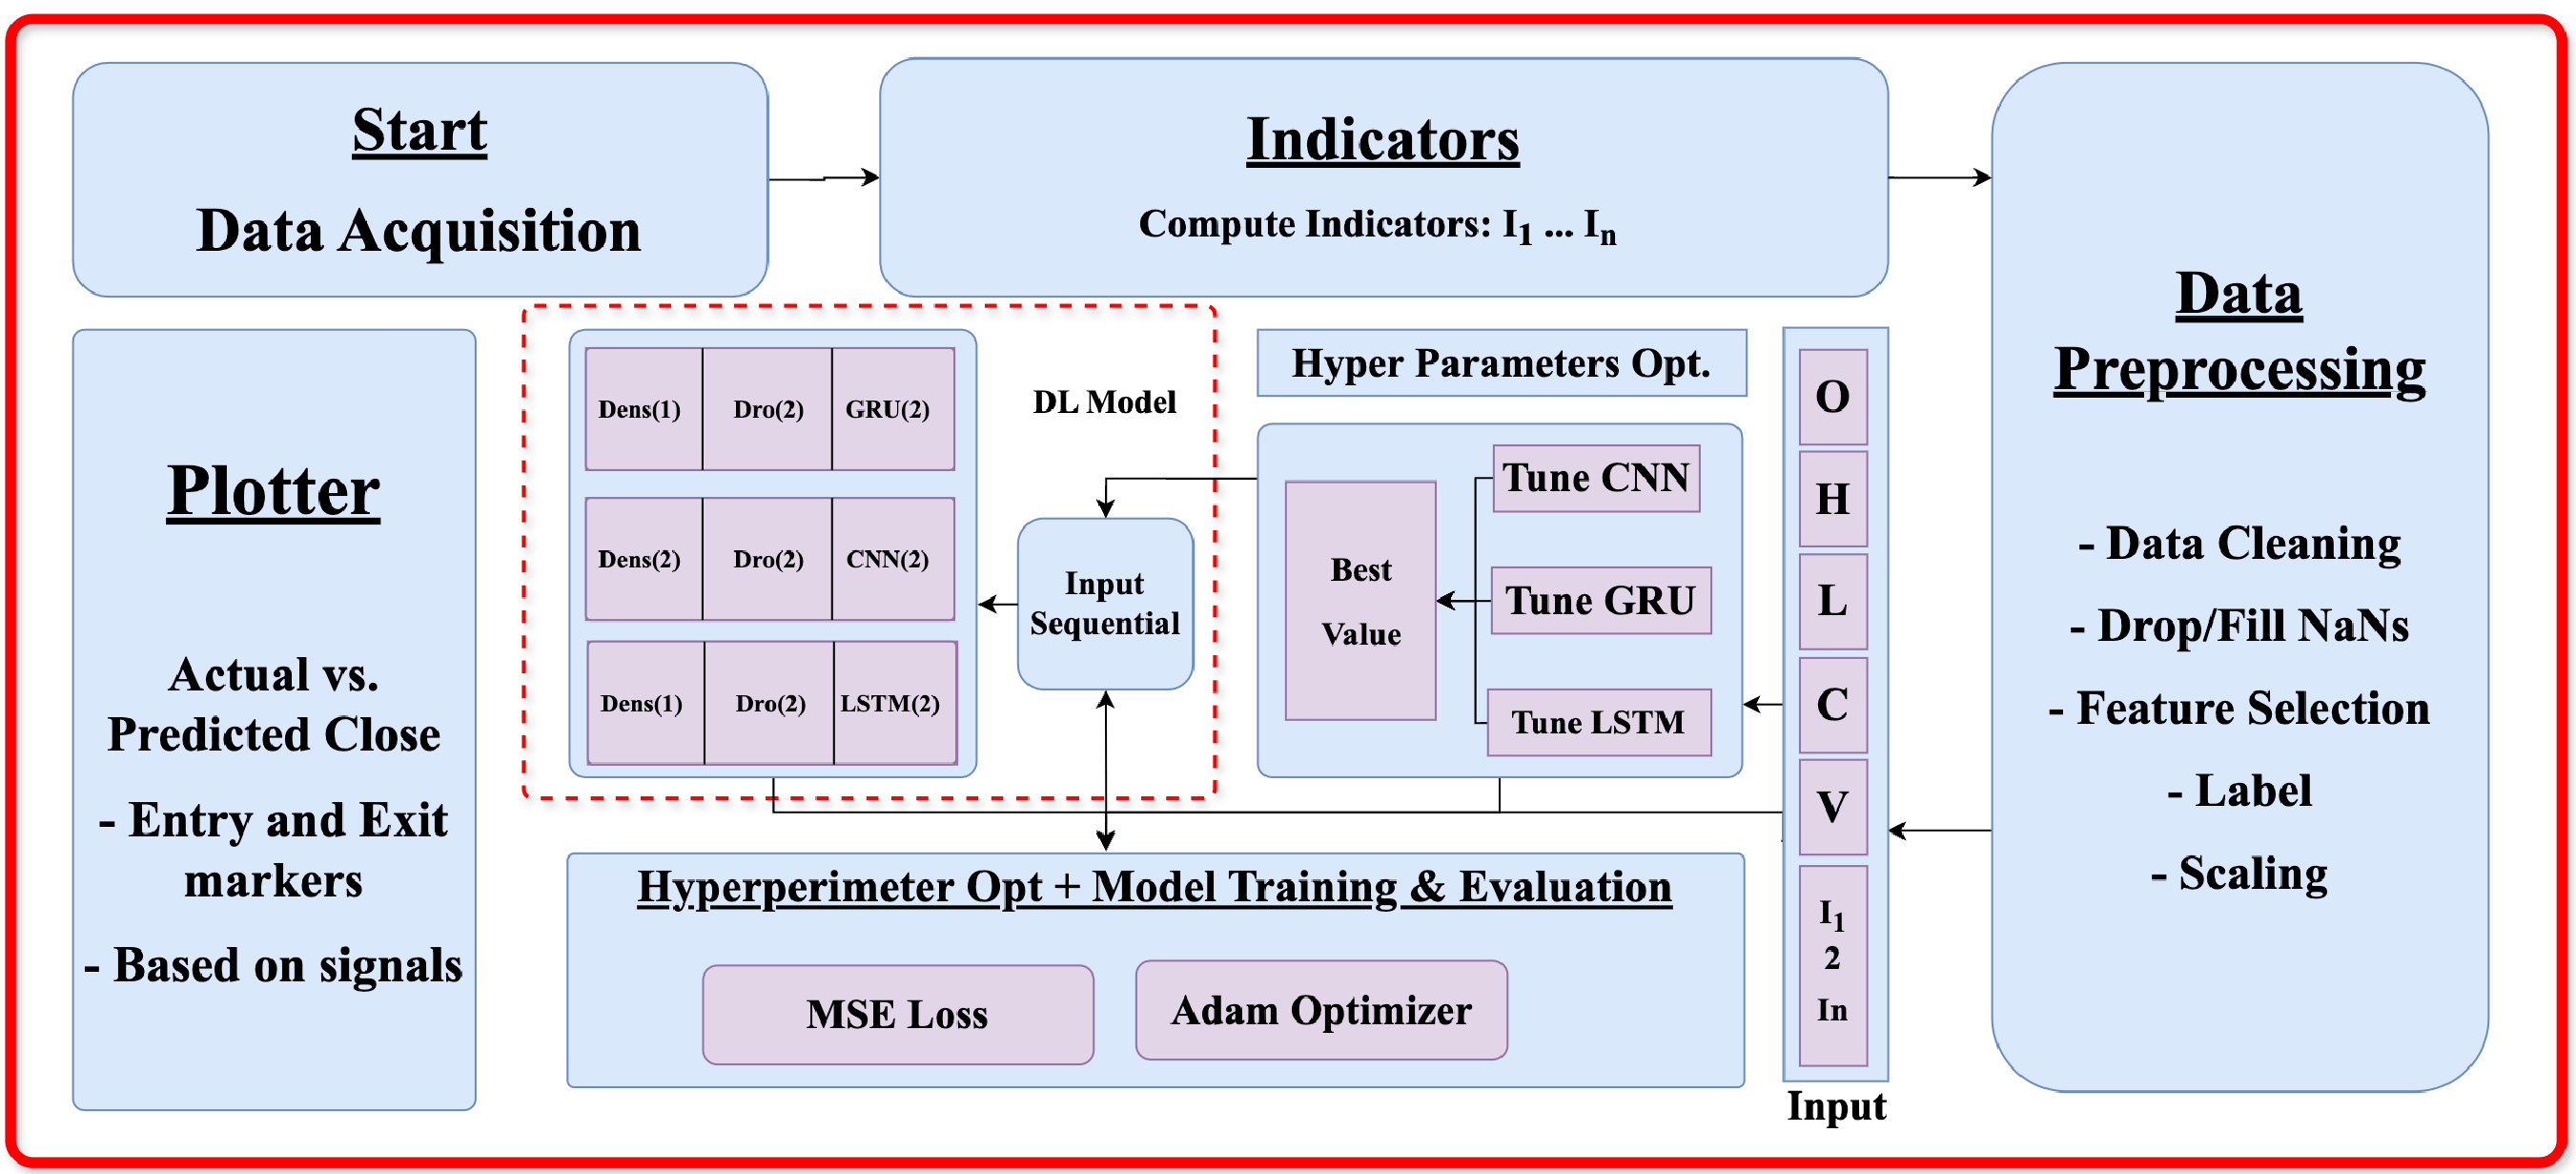
\includegraphics[width=1\textwidth, height=12cm]{DL-Architecture}
    \caption{DL Architecture}
    \label{fig:DLArchitecture}
\end{figure}

\subsection{Data Collection}
This study employs historical NVDA stock data obtained from a credible financial database (e.g. Yahoo Finance or Quandl), spanning a 15-year timeframe (2010-2025) at daily frequency. The dataset contains important financial metrics: open, high, low, close prices and volume of trade. This period covers S\&P500’sprice action characterized by the volatility caused by GPU innovations and trends surrounding AI, and therefore serves as an apt candidate for testing DL models. Here, the data obtained in a pandas dataframe format, and so it will be compatible with the next processing steps.

\subsection{Data Preparation}
The next stage involves a ton of data preprocessing to ensure model robustness as stock price is non-stationary. Sort it by date first and then do forward and backward fill (ffill and bfill) for the missing values. Normalization for each individual ticker is done using `MinMaxScaler` from the scikit-learn package, so the price range for each stock is rescaled separately to alleviate the common problem of non-stationarity in time-series forecasting [3]. From computed technical indicators, we include derived features, e.g., average price so far after a day weighted by frequency (volume-weighted average price), with a custom `StockIndicators` class (i.e., 20 day moving average). We tune a significant hyperparameter called the look back period, determining a time frame between 10 and up to 120 days to constitute a salient feature space which retains relevant historical context, white removing nulls etc, and finally resetting the index of dataset.

\subsection{Model Architecture}
Understanding multivariate relationships among multiple variables, such as open, high, low, close, and volume, are essential for stock price prediction. Each model, including LSTM, GRU, and CNN, are equipped with configurable numbers of underlying layers, which can be stacked with recurrent or convolutional units, followed by a dropout for regularization and a dense output layer, and is configured to generate robust forecasting models via an Adam optimizer, mean squared error with an early-stopping generalization performance threshold.\\

\textbf{Note: } All model - Input data is (OHLCV DataFrame), $L$ (lookback), $\Theta = \{ u, d \}$, $\mathcal{E}$ (epochs), $B$ (batch size) and Output is Price predictions.

\begin{itemize}
    \item \textbf{LSTM:} The model has two stacked layers with a dropout layer, after each layer to help prevent overfitting where some neurons are randomly deactivated during training. The first layer is an LSTM with a configurable number of units (50), and it returns sequences to the next layer, and the second layer also an LSTM (with 50 units) returns a single vector. Dropout layers apply a fraction of inputs with a configurable minimum (defaulting to 0.2). This is followed by a Dense output layer with a single unit which generates the stock price prediction.
    
    \begin{table}[h]
    \small
    \centering
    \begin{tabular}{|p{10cm}|}
    \hline
    \textbf{Algorithm 2: LSTM Stock Price Prediction} \\
    \hline
    1: \textbf{for each} $t \in [L, \text{len}(data))$ \textbf{do} \\
    2: \quad Define BuildLSTM($\Theta$, $L$, data): \\
    3: \quad\quad $\mathcal{M}$ = Sequential([Input($L$, 1), LSTM($\Theta.u$, True), Dropout($\Theta.d$), LSTM($\Theta.u$, False), Dropout($\Theta.d$), Dense(1)]); \\
    4: \quad\quad $\mathcal{M}$.compile(Adam(0.001), 'mse'); \\
    5: \quad\quad X, y = PrepareSequenceData(data, $L$); \\
    6: \quad\quad $\mathcal{M}$.fit(SplitData(X, y)[0:2], $\mathcal{E}$, $B$); \\
    7: \quad\quad \textbf{return} $\mathcal{M}$.predict(SplitData(X, y)[2]); \\
    8: \quad predictions[$t$] = BuildLSTM($\Theta$, $L$, data); \\
    9: \textbf{return} predictions \\
    \hline
    \end{tabular}
    \caption{LSTM Model for Stock Price Prediction}
    \label{tab:lstm_predictor}
    \end{table}
    

    \item \textbf{GRU: } We optimize two stacked layers of GRU model along with a dropout layer appended to each GRU layer for preventing overfitting and improving generalization. In the first: return sequences, in a configurable number (50 default), and in the second: return sequences to a single output. Dropout layers make use of a user configurable rate (0.2 by default). A Dense output layer with a single unit subsequently maps to future stock prices.
    
    \begin{table}[h]
    \small
    \centering
    \begin{tabular}{|p{10cm}|}
    \hline
    \textbf{Algorithm 3: GRU Stock Price Prediction} \\
    \hline
    1: \textbf{for each} $t \in [L, \text{len}(data))$ \textbf{do} \\
    2: \quad Define BuildGRU($\Theta$, $L$, data): \\
    3: \quad\quad $\mathcal{M}$ = Sequential([Input($L$, 1), GRU($\Theta.u$, True), Dropout($\Theta.d$), GRU($\Theta.u$, False), Dropout($\Theta.d$), Dense(1)]); \\
    4: \quad\quad $\mathcal{M}$.compile(Adam(0.001), 'mse'); \\
    5: \quad\quad X, y = PrepareSequenceData(data, $L$); \\
    6: \quad\quad $\mathcal{M}$.fit(SplitData(X, y)[0:2], $\mathcal{E}$, $B$); \\
    7: \quad\quad \textbf{return} $\mathcal{M}$.predict(SplitData(X, y)[2]); \\
    8: \quad predictions[$t$] = BuildGRU($\Theta$, $L$, data); \\
    9: \textbf{return} predictions \\
    \hline
    \end{tabular}
    \caption{GRU Model for Stock Price Prediction}
    \label{tab:gru_predictor}
    \end{table}
    
    \item \textbf{CNN: }  The first Conv1D layer has a predetermined number of filters (default=32) and kernel size (default=3) and applies ReLU activation over a subsequent dropout layer (rate custom; default=0.2). The second Conv1D layer has a predetermined number of filters (default=32) and kernel size (default=3) with ReLU activation. An output dense layer with a single unit creates the stock price prediction, capturing complex nonlinear relationships in the data.
    
    \begin{table}[h]
    \tiny
    \centering
    \begin{tabular}{|p{10cm}|}
    \hline
    \textbf{Algorithm 4: CNN Stock Price Prediction} \\
    \hline
    1: \textbf{for each} $t \in [L, \text{len}(data))$ \textbf{do} \\
    2: \quad Define BuildCNN($\Theta$, $L$, data): \\
    3: \quad\quad $\mathcal{M}$ = Sequential([Input($L$, 1), Conv1D($\Theta.f_1$, $\Theta.k_1$, 'relu'), Dropout($\Theta.d$), Conv1D($\Theta.f_2$, $\Theta.k_2$, 'relu'), Flatten(), Dense($\Theta.u$, 'relu'), Dropout($\Theta.d$), Dense(1)]); \\
    4: \quad\quad $\mathcal{M}$.compile(Adam(0.001), 'mse'); \\
    5: \quad\quad X, y = PrepareSequenceData(data, $L$); \\
    6: \quad\quad $\mathcal{M}$.fit(SplitData(X, y)[0:2], $\mathcal{E}$, $B$); \\
    7: \quad\quad \textbf{return} $\mathcal{M}$.predict(SplitData(X, y)[2]); \\
    8: \quad predictions[$t$] = BuildCNN($\Theta$, $L$, data); \\
    9: \textbf{return} predictions \\
    \hline
    \end{tabular}
    \caption{CNN Model for Stock Price Prediction}
    \label{tab:cnn_predictor}
    \end{table}

\end{itemize}

\subsection{Hyperparameter Tuning: } Since deep learning models must learn on sequential data such as OHLCV, hyperparameter tuning should be an essential component of producing performant models for stock price prediction, specifically for OHLCV data [4] [5]. The \textbf{HyperparameterTuner} class utilizes Random Search to discover optimal LSTM, GRU, and CNN hyper-parameters, achieving a more effective model complexity vs generalization trade-off by exhaustively searching through parameter spaces.

\begin{equation}
\textbf{Hyperparameter optimization: } \Theta^* = \arg\min_{\Theta \in \mathcal{S}_\Theta} L(M_\Theta(X_t, y_t), X_v, y_v)
\label{math_hyperparameter_optimization}
\end{equation}

\begin{equation}
\textbf{Minimize validation loss: } L(M_\Theta, X_v, y_v) = \frac{1}{n} \sum_{i=1}^{n} (y_{v,i} - M_\Theta(X_t, y_t)(X_{v,i}))^2
\label{math_minimize_validation_loss}
\end{equation}

\begin{equation}
\textbf{Output: } \hat{y} = \frac{1}{|\mathcal{M}|} \sum_{M_m \in \mathcal{M}} M_m(X; \Theta_m^*)
\label{math_dl_output}
\end{equation}

\begin{table}[h]
\small
\centering
\begin{tabular}{|p{14cm}|}
\hline
\textbf{Algorithm 5: Hyperparameter Tuning (LSTM/GRU/CNN)} \\
\hline
\textbf{Input:} $X_t, y_t$ (train), $X_v, y_v$ (val), $L$ (lookback), $\mathcal{E}$ (epochs), $T$ (trials), $M_{type}$ (LSTM, GRU, or CNN) \\
\textbf{Output:} $\Theta^*$ (best params) \\
\hline
1: Define $M_\Theta$ based on $M_{type}$: \\
2: \quad \textbf{if} $M_{type}$ = LSTM or GRU: \\
3: \quad\quad $M_\Theta$: [$M_{type}$($u$, True, ($L$, 1)) $\rightarrow$ Dropout($d$) $\rightarrow$ $M_{type}$($u$) $\rightarrow$ Dropout($d$) $\rightarrow$ Dense(1)]; \\
4: \quad\quad $\mathcal{S}_\Theta = \{ u \in [20, 200], d \in \{0, 0.2, 0.5\} \}$; \\
5: \quad \textbf{else if} $M_{type}$ = CNN: \\
6: \quad\quad $M_\Theta$: [Conv1D($f_1$, $k_1$, 'relu', ($L$, 1)) $\rightarrow$ Dropout($d$) $\rightarrow$ Conv1D($f_2$, $k_2$, 'relu') $\rightarrow$ Flatten() $\rightarrow$ Dense($u$, 'relu') $\rightarrow$ Dropout($d$) $\rightarrow$ Dense(1)]; \\
7: \quad\quad $\mathcal{S}_\Theta = \{ f_1, f_2 \in [16, 128], k_1, k_2 \in [2, 5], u \in [20, 200], d \in \{0, 0.2, 0.5\} \}$; \\
8: \quad $L_\Theta = L(M_\Theta(X_t, y_t, \mathcal{E}), X_v, y_v)$; \\
9: \textbf{for} $i = 1$ \textbf{to} $T$ \textbf{do} \\
10: \quad Sample $\Theta_i \sim \mathcal{S}_\Theta$; \\
11: \quad Compute $L_{\Theta_i}$; \\
12: $\Theta^* \leftarrow \arg\min_{\Theta_i} L_{\Theta_i}$; \\
13: \textbf{return} $\Theta^*$ \\
\hline
\end{tabular}


\caption{Hyperparameter Tuning for LSTM, GRU, CNN}
\label{tab:dynamic_dl_tuner}
\end{table}
The tuning process starts with a unified initialization, passing in training data ($X_{train}$, $y_{train}$), validation data  ($X_{val}$, $y_{val}$), a lookback window ($L$), and a default of 100 epochs ($\mathcal{E}$). For tuning the respective models—LSTM, GRU, and CNN—they each have a single tuning method  (\texttt{tune\_lstm}, \texttt{tune\_gru}, \texttt{tune\_cnn}), which uses \textbf{KerasTuners} \textbf{RandomSearch} certain  (default $T = 10$) number of times (\texttt{val\_loss}) to minimize.

\subsection{Model Training and Combination}

The \texttt{CombinedModel} class is training three models — LSTM, GRU, and CNN — to predict stock prices from OHLCV data. It starts from selecting the models we want to use, such as LSTM or CNN, by model\_types. Here each model has a lookback window (default 60) that looks to see what past data points feel like. 

\begin{equation}
\textbf{Train models: }\Theta_m^* = \arg\min_{\Theta_m \in \mathcal{S}_{\Theta_m}} L(M_m(X_t, y_t; \Theta_m), X_v, y_v)
\label{math_dl_train_models}
\end{equation}

\begin{table}[h]
\small
\centering
\begin{tabular}{|p{10cm}|}
\hline
\textbf{Algorithm 6: CombinedModel Training} \\
\hline
\textbf{Input:} $X_t, y_t$ (OHLCV train data), $X_v, y_v$ (val data), $L$ (lookback), $\mathcal{M}$ (model types), $\Theta_m$ (hyperparams), $\mathcal{E}$ (epochs), $B$ (batch size) \\
\textbf{Output:} Trained models $\mathcal{M}^*$ \\
\hline
1: \textbf{for each} $M_m \in \mathcal{M}$ \textbf{do} \\
2: \quad Define TrainModel($M_m$, $\Theta_m$, $X_t$, $y_t$): \\
3: \quad\quad $\mathcal{M}_m$ = ModelFactory($M_m$, $L$, $\Theta_m$); \\
4: \quad\quad $\mathcal{M}_m$.compile(Adam(0.001), 'mse'); \\
5: \quad\quad $\mathcal{M}_m$.fit($X_t$, $y_t$, $\mathcal{E}$, $B$, val=($X_v$, $y_v$), early\_stop=10); \\
6: \quad\quad \textbf{return} $\mathcal{M}_m$; \\
7: \quad $\mathcal{M}_m^*$ = TrainModel($M_m$, $\Theta_m$, $X_t$, $y_t$); \\
8: \quad Store $\mathcal{M}_m^*$ in $\mathcal{M}^*$, loss in History; \\
9: \textbf{return} $\mathcal{M}^*$ \\
\hline
\end{tabular}
\caption{CombinedModel Training Pseudocode}
\label{tab:combined_dl_model_train}
\end{table}

In specify options, such as number of units or dropout rates, hyperparams too, but if we don’t, it defaults to an empty set. Training begins with train, where we provide the training data — OHLCV prices to use as input and future prices as the output target. It trains each model for as many as 100 epochs (rounds), adjusting them in batches of 128 to pick up patterns. It breaks off 20\% of the data to use a separate validation set to see how well the model is doing. We stop early training if there is no drop in error for 10 rounds, save the model with the smallest error seen. The same for each model call by looping. When finished, the models are saved in the provided folder to use in the future. Models training progress (loss scores) all feed we can find into the history. Then the models delevloper tema can find out by averaging their outputs to make predictions, and accuricy.

\subsection{Result: Signal Generation and Backtesting}
The \texttt{StockTrader} class coordinates stock trading by linking important components. DataProcessor processes OHLCV (2010-2024, day timeframe), determines a lookback period (e.g. 60 days), and separates into sets: X\_train, X\_test. It tries lookback values of 10 to 120 days and choose the best based on validation loss. On top of that, \texttt{HyperparameterTuner} refines the LSTM, GRU, and CNN models. For GRU and LSTM it iterates through units (20 to 200) and dropout rates (0, 0.2, 0.5), and for CNN through filters (16 to 128) and kernel sizes (2 to 5), executing 5 trials in order to get the lowest validation error.

\begin{table}[h]
\small
\centering
\caption{Backtesting Results for StockTrader with CNN, GRU, and LSTM Models}
\label{tab:backtest_results}
\begin{tabular}{ll}
\toprule
\textbf{Metric} & \textbf{Value} \\
\midrule
Ticker (Models) & GSPC (CNN, GRU, LSTM) \\
Initial Balance & \$5,000.00 \\
Final Balance & \$5,186.55 \\
Total Trades & 20 \\
Max Drawdown & 0.0325 \\
Sharpe Ratio & 0.3626 \\
Model Testing Data Time Period & 2015-01 to 2024-09 \\
Test Trading Time Period & 2024-10 to 2025-02 \\
\bottomrule
\end{tabular}
\end{table}

Afterward, the \texttt{CombinedModel} utilizes the tuned settings to fit these models with full training data (100 rounds (epochs) with batches of 128) and combines their predictions (combined\_pred) from LSTM, GRU, and CNN. Enter the \texttt{Backtester} which takes predictions from \texttt{SignalGenerator} and converts them into buy (1), sell (-1) or hold (0) signals based on a 1\% price change, simulating trades on the test data, starting with \$5000 and a \$0.01 cost while logging balances and trades. Eventually \texttt{PerformanceAnalyzer} checks results (max\_drawdown, sharpe ratio, etc), and creates plots for prices, signals, and performance.

\begin{figure}[htbp]
    \centering
    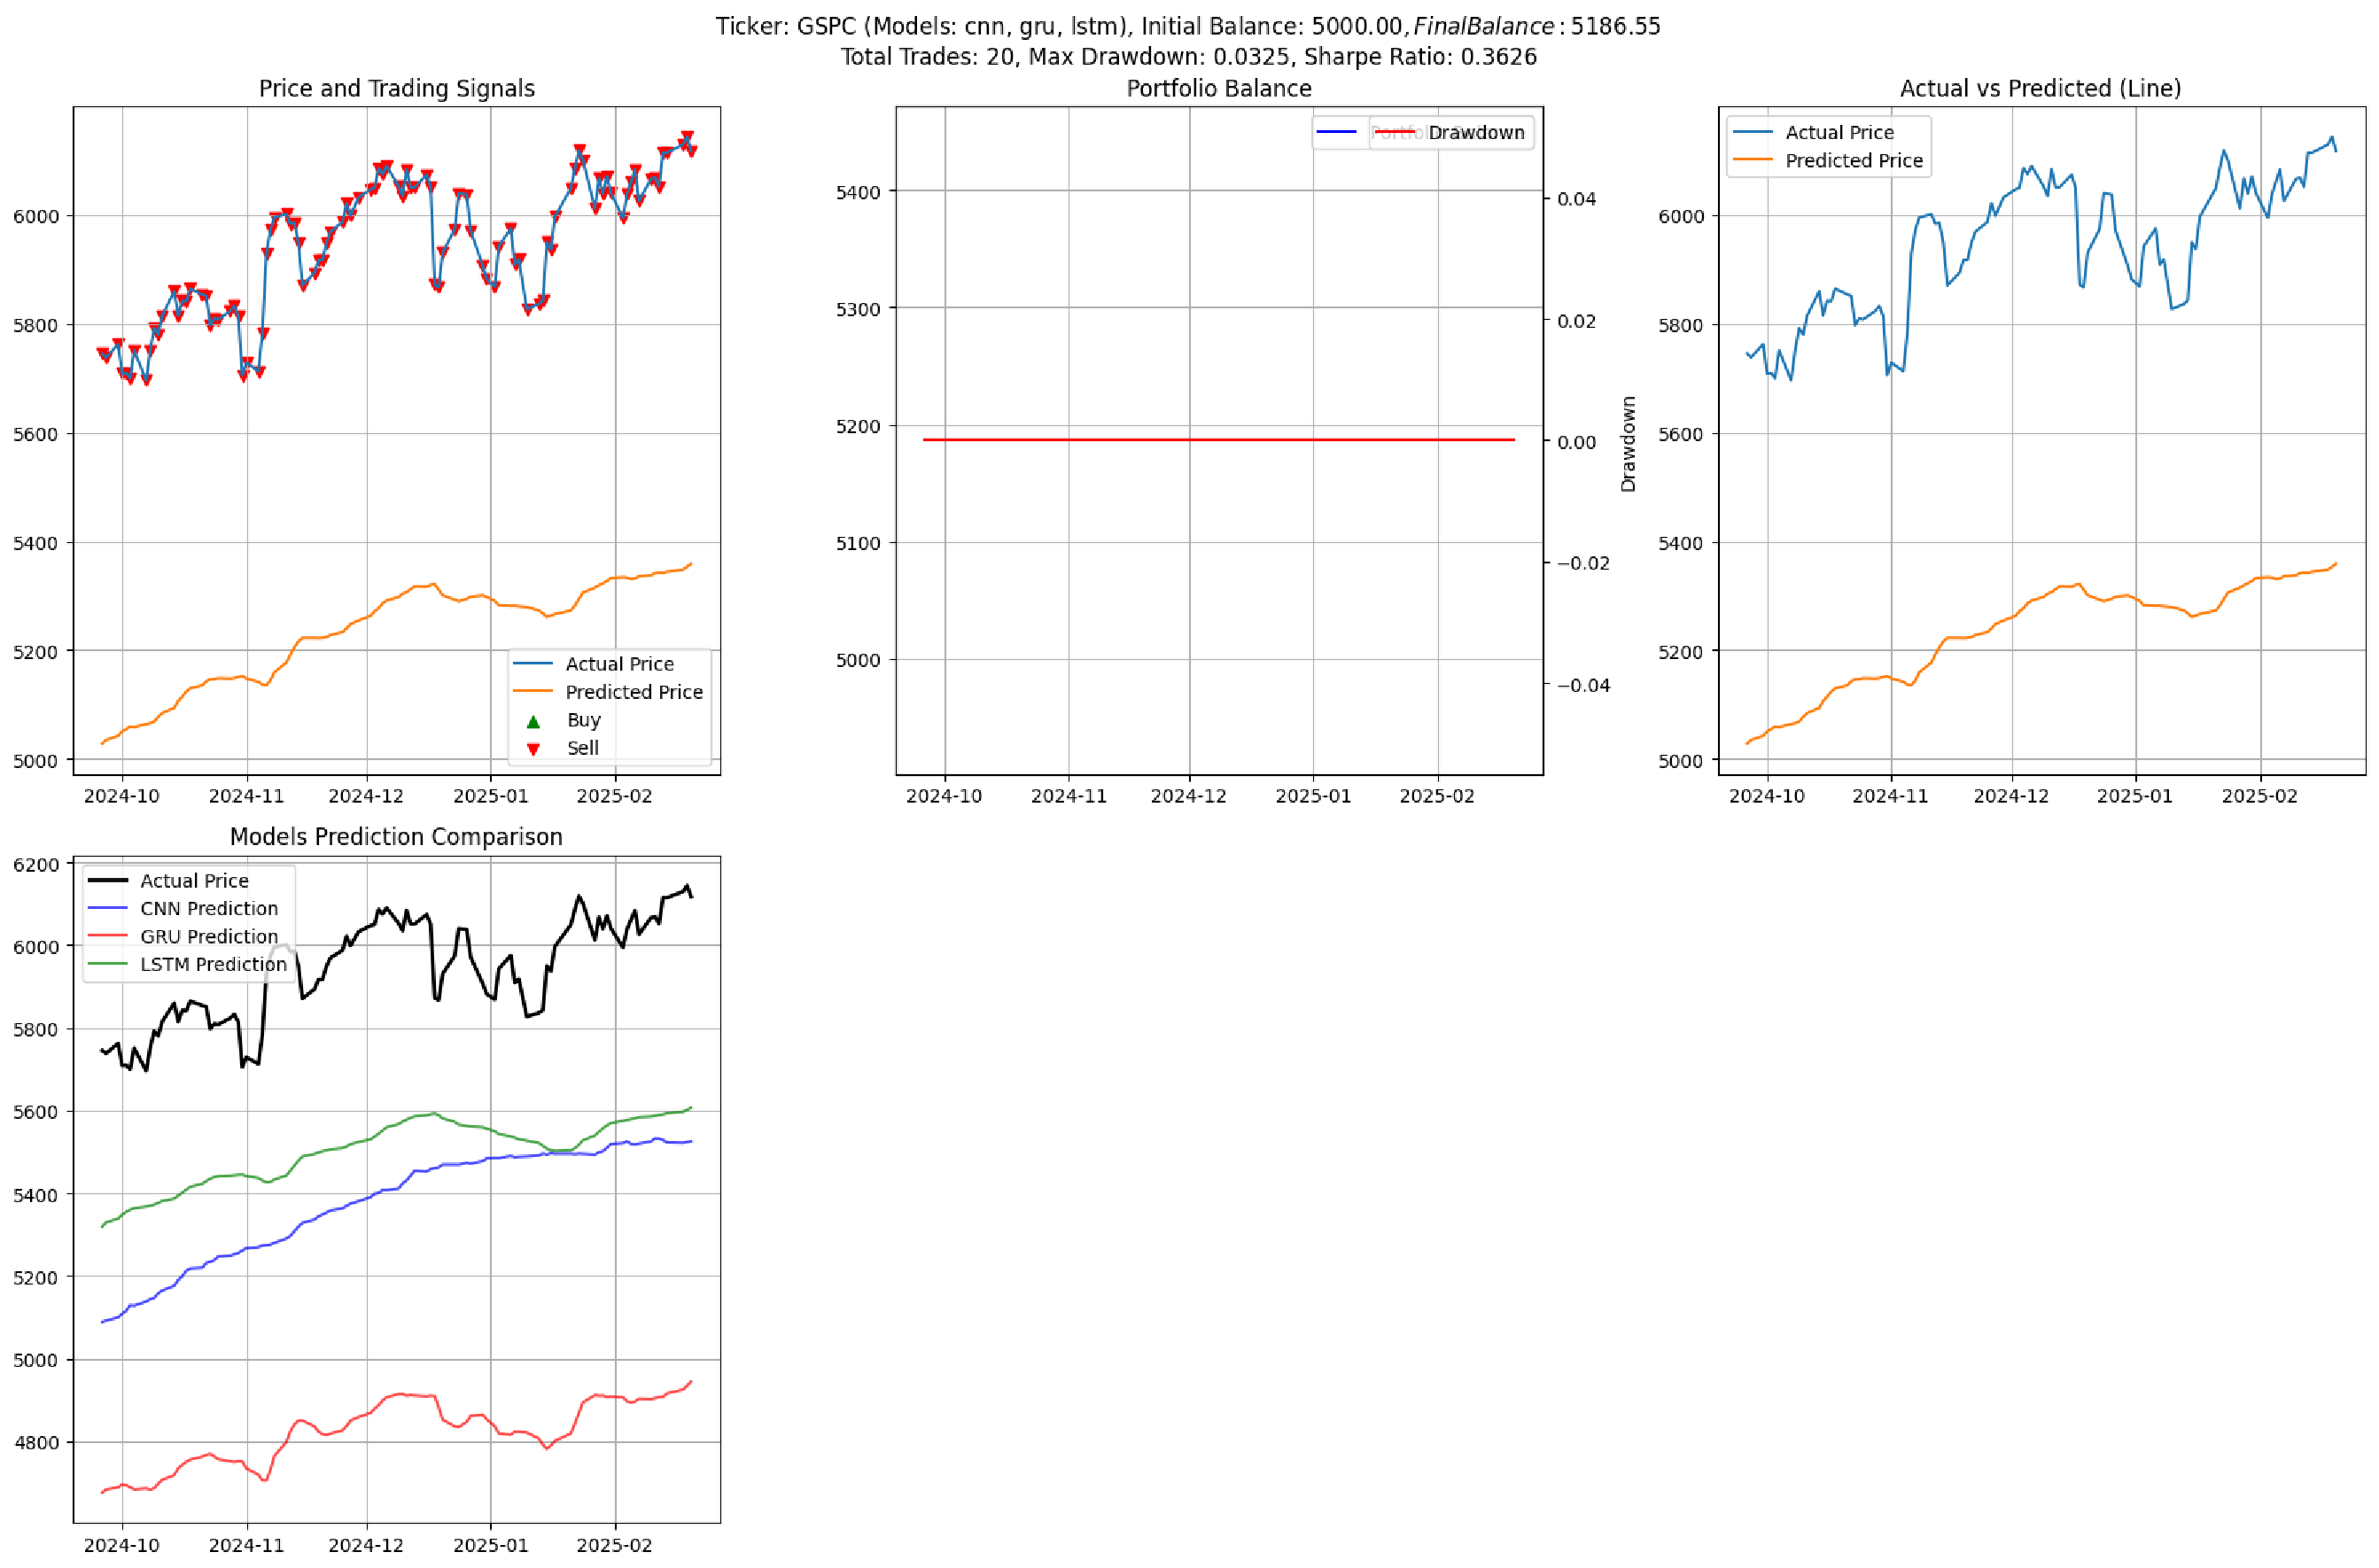
\includegraphics[width=1\textwidth, height=6.5cm]{DL-GRU-CNN-LSTM}
    \caption{GRU, CNN, and LSTM Model Performance}
    \label{fig:dl_models_performance}
\end{figure}